\documentclass[conference,compsoc]{IEEEtran}
\usepackage[T1]{fontenc}
\usepackage{amsmath,amssymb,amsthm,booktabs,graphicx,array}
\usepackage[hidelinks,pdfauthor={},pdftitle={Certified Evaluation of Autonomous Cyber Defenders}]{hyperref}
\usepackage{microtype}
\usepackage{placeins}
\makeatletter\let\tableinput\@@input\makeatother
% Generated; do not edit.
\newcommand{\AhChampBest}{0.70}
\newcommand{\AhChampBreach}{0.68}
\newcommand{\AhChampEps}{40}
\newcommand{\AhChampExpThree}{0.23}
\newcommand{\AhChampHi}{0.93}
\newcommand{\AhChampLo}{0.39}
\newcommand{\AhChampRand}{0.17}
\newcommand{\AhChampShare}{98}
\newcommand{\AhFixBest}{0.00}
\newcommand{\AhFixBreach}{0.00}
\newcommand{\AhFixEps}{40}
\newcommand{\AhFixExpThree}{0.00}
\newcommand{\AhFixHi}{0.19}
\newcommand{\AhFixLo}{0.00}
\newcommand{\AhFixRand}{0.00}
\newcommand{\AhFixShare}{10}
\newcommand{\AhRestoreBest}{0.17}
\newcommand{\AhRestoreBreach}{0.17}
\newcommand{\AhRestoreEps}{40}
\newcommand{\AhRestoreExpThree}{0.09}
\newcommand{\AhRestoreHi}{0.44}
\newcommand{\AhRestoreLo}{0.00}
\newcommand{\AhRestoreRand}{0.07}
\newcommand{\AhRestoreShare}{88}
\newcommand{\AsChampBest}{0.67}
\newcommand{\AsChampBreach}{0.30}
\newcommand{\AsChampEps}{30}
\newcommand{\AsChampExpThree}{0.23}
\newcommand{\AsChampHi}{0.65}
\newcommand{\AsChampLo}{0.00}
\newcommand{\AsChampRand}{0.17}
\newcommand{\AsChampShare}{57}
\newcommand{\AsFixBest}{0.00}
\newcommand{\AsFixBreach}{0.00}
\newcommand{\AsFixEps}{30}
\newcommand{\AsFixExpThree}{0.00}
\newcommand{\AsFixHi}{0.26}
\newcommand{\AsFixLo}{0.00}
\newcommand{\AsFixRand}{0.00}
\newcommand{\AsFixShare}{27}
\newcommand{\AsRestoreBest}{0.17}
\newcommand{\AsRestoreBreach}{0.17}
\newcommand{\AsRestoreEps}{30}
\newcommand{\AsRestoreExpThree}{0.09}
\newcommand{\AsRestoreHi}{0.49}
\newcommand{\AsRestoreLo}{0.00}
\newcommand{\AsRestoreRand}{0.07}
\newcommand{\AsRestoreShare}{83}
\newcommand{\AtkCost}{1.20}
\newcommand{\AtkModels}{2}
\newcommand{\CgChampAdaptBreach}{24}
\newcommand{\CgChampAdaptDelayed}{79}
\newcommand{\CgChampAdaptUp}{0.36}
\newcommand{\CgChampAllBreachCert}{0.76}
\newcommand{\CgChampDelayedBreach}{64}
\newcommand{\CgChampDelayedLow}{0.51}
\newcommand{\CgChampDelayedReward}{-91.0}
\newcommand{\CgChampDelayedUp}{0.74}
\newcommand{\CgChampRankCert}{4}
\newcommand{\CgChampRankMean}{1}
\newcommand{\CgChampSeenBreachUp}{0.04}
\newcommand{\CgChampSeenReward}{-5.6}
\newcommand{\CgDefenders}{5}
\newcommand{\CgEpisodeBound}{474}
\newcommand{\CgEpisodes}{200}
\newcommand{\CgFixAdaptUp}{0.13}
\newcommand{\CgFixAllBreachCert}{0.04}
\newcommand{\CgFixDelayedReward}{-4.3}
\newcommand{\CgLlmCost}{23.74}
\newcommand{\CgRemoveAllBreachCert}{0.71}
\newcommand{\CgRestoreAllBreachCert}{0.22}
\newcommand{\CgRestoreSeenReward}{-20.6}
\newcommand{\CgStepBound}{15.8}
\newcommand{\CgSteps}{30}
\newcommand{\CgStopMax}{149}
\newcommand{\CgStopMedian}{38}
\newcommand{\CgStopMin}{12}
\newcommand{\CgStopPairs}{20}
\newcommand{\CgStopResolved}{18}
\newcommand{\CgValBlinePort}{-5.24}
\newcommand{\CgValBlinePub}{-3.41}
\newcommand{\CgValEpisodes}{1000}
\newcommand{\CgValMeanderPort}{-5.58}
\newcommand{\CgValMeanderPub}{-5.54}
\newcommand{\HnAllBreachCert}{0.55}
\newcommand{\HnBlineBreach}{11}
\newcommand{\HnBreaches}{7}
\newcommand{\HnCalls}{3300}
\newcommand{\HnCertCost}{52}
\newcommand{\HnCertHours}{22}
\newcommand{\HnCost}{7.21}
\newcommand{\HnCostEp}{0.07}
\newcommand{\HnDelayedBreach}{14}
\newcommand{\HnDelayedReward}{-17.0}
\newcommand{\HnEpisodes}{110}
\newcommand{\HnInvalid}{0}
\newcommand{\HnMax}{28}
\newcommand{\HnMinutes}{1.6}
\newcommand{\HnPairN}{28}
\newcommand{\HnPairOnlyChamp}{16}
\newcommand{\HnPairOnlyLlm}{1}
\newcommand{\HnPairP}{0.000}
\newcommand{\HnPairVerdict}{unresolved}
\newcommand{\HnPer}{27}
\newcommand{\HnSeenReward}{-15.7}
\newcommand{\HtAllBreachCert}{1.00}
\newcommand{\HtBlineBreach}{40}
\newcommand{\HtBreaches}{3}
\newcommand{\HtCalls}{600}
\newcommand{\HtCertCost}{231}
\newcommand{\HtCertHours}{127}
\newcommand{\HtCost}{5.77}
\newcommand{\HtCostEp}{0.29}
\newcommand{\HtDelayedBreach}{20}
\newcommand{\HtDelayedReward}{-17.5}
\newcommand{\HtEpisodes}{20}
\newcommand{\HtInvalid}{1}
\newcommand{\HtMax}{5}
\newcommand{\HtMinutes}{9.5}
\newcommand{\HtPairN}{5}
\newcommand{\HtPairOnlyChamp}{2}
\newcommand{\HtPairOnlyLlm}{0}
\newcommand{\HtPairP}{0.500}
\newcommand{\HtPairVerdict}{unresolved}
\newcommand{\HtPer}{5}
\newcommand{\HtSeenReward}{-16.4}
\newcommand{\SnAllBreachCert}{1.00}
\newcommand{\SnBlineBreach}{0}
\newcommand{\SnBreaches}{0}
\newcommand{\SnCalls}{1020}
\newcommand{\SnCertCost}{253}
\newcommand{\SnCertHours}{36}
\newcommand{\SnCost}{10.76}
\newcommand{\SnCostEp}{0.32}
\newcommand{\SnDelayedBreach}{0}
\newcommand{\SnDelayedReward}{-11.3}
\newcommand{\SnEpisodes}{34}
\newcommand{\SnInvalid}{3}
\newcommand{\SnMax}{10}
\newcommand{\SnMinutes}{2.7}
\newcommand{\SnPairN}{10}
\newcommand{\SnPairOnlyChamp}{7}
\newcommand{\SnPairOnlyLlm}{0}
\newcommand{\SnPairP}{0.016}
\newcommand{\SnPairVerdict}{unresolved}
\newcommand{\SnPer}{7}
\newcommand{\SnSeenReward}{-9.4}

\newtheorem{proposition}{Proposition}

\begin{document}
\title{Certified Evaluation of Autonomous Cyber Defenders:\\
A Five-Step Delay Breaks the CAGE-2 Champion}
\author{\IEEEauthorblockN{Anonymous Author(s)}\IEEEauthorblockA{Anonymized for double-blind review}}
\maketitle

\begin{abstract}
Autonomous cyber defenders, from reinforcement-learning (RL) agents to language-model
agents, are compared by their mean reward over a fixed number of episodes against the
scripted attackers they were built for. Such scores carry no guarantee and say nothing
about attackers outside that set. We propose a \emph{certified evaluation} protocol:
distribution-free confidence bounds on a defender's reward and on the probability that
the mission-critical server is breached, valid simultaneously at every number of
episodes (so evaluation may stop as soon as a verdict is reached), valid against an
attacker that adapts across episodes, and combined into a joint worst case over a set of
attackers that includes ones the defender has not seen. Applied to CAGE Challenge~2,
the protocol shows that the challenge's winning RL agent, which is never breached by
the two official attackers (certified breach rate at most \CgChampSeenBreachUp), is
breached in \CgChampDelayedBreach\% of episodes when the official B\_line attacker
simply waits one to five steps before starting: its attacker fingerprint misfires and it
falls back to doing nothing. An adaptive attacker finds this on its own. The winner ranks
first of \CgDefenders{} defenders by mean reward and \CgChampRankCert{}th by certified worst case, and
a one-line change, which the certificate pointed to, restores a certified breach rate of
at most \CgFixAllBreachCert{} on every attacker. A language-model attacker (Claude Haiku~4.5),
told only to find what breaches the defender, discovers the same blind spot unaided:
against the winner it breaches \AhChampBreach{} of episodes --- matching the best fixed
strategy in hindsight (\AhChampBest) and far above uniform choice (\AhChampRand) --- yet
against the repaired winner it breaches \AhFixBreach. Given instead CybORG's raw actions, a
language model operates the full kill chain unaided but, attacking at once, rarely
rediscovers the timing weakness the selector sought out; the blind spot holds across a whole delay family, and the
protocol carries over to a second environment (CAGE Challenge~1). Language-model defenders do not share the
winner's blind spot: Claude Sonnet~5 was breached in \SnBreaches{} of \SnEpisodes{} episodes
and Claude Haiku~4.5 in \HnDelayedBreach\% of delayed-attacker episodes. Certifying them to
the winner's precision, however, would take hundreds of dollars and tens of hours of
evaluation per model; we quantify that cost.
\end{abstract}

\begin{IEEEkeywords}
autonomous cyber defense, CybORG, CAGE challenge, LLM agents, reinforcement learning,
evaluation, anytime-valid inference, robustness
\end{IEEEkeywords}

\section{Introduction}
Autonomous defense agents are now trained and benchmarked in cyber-operations
simulators~\cite{standen2021cyborg}, and language-model (LLM) agents have joined the
reinforcement-learning (RL) agents that dominate the leaderboards~\cite{castro2025llm}.
The CAGE challenges rank submissions by mean reward against the same rule-based
attackers used during development, which rewards solutions fitted to known
adversaries~\cite{king2025graph}. Reported scores are means and standard deviations over
a fixed number of episodes; they carry no guarantee, and they are silent about what an
attacker outside the evaluation set would do.

We ask what a defender can be \emph{certified} to achieve. Our protocol gives, for each
defender and attacker, confidence bounds on the expected episode reward and on the
probability that the operational server is breached that are distribution-free (they use
only the known range of the outcome), valid simultaneously at every number of episodes
(the evaluator may look after every episode and stop as soon as the answer is settled),
and, for an attacker that adapts across episodes, valid for the running average of what
the attacker achieves. A defender's certified worst case is the least favourable bound
over a set of attackers that deliberately includes ones it was not built against.

\paragraph{Contributions}
(i) A certified evaluation protocol for autonomous defenders with time-uniform,
distribution-free bounds, a martingale variant for adaptive attackers, and a joint worst
case over attackers (Section~\ref{sec:protocol}). (ii) A faithful, framework-free port
of the CAGE Challenge~2 winning agent and two unseen attackers that only re-sequence the
official attackers' actions (Section~\ref{sec:setup}). (iii) The finding that the
winner's guarantees do not transfer: a delay of one to five steps defeats it, an
adaptive attacker discovers this unaided, the certified ranking reverses, and a one-line
repair restores the guarantee (Section~\ref{sec:results}). (iv) Claude defenders
evaluated under the same protocol, with and without extended thinking, and the episode
and dollar cost of certifying an LLM defender. (v) A language-model attacker that, given
only the goal of breaching the defender, autonomously finds and exploits the winner's
blind spot yet is defeated by the one-line repair; and a primitive-action variant that
issues raw CybORG actions and operates the full kill chain unaided, separating operating
an attack from discovering the timing weakness. (vi) Evidence the finding is robust: the
blind spot holds across a parameterized delay family and the protocol carries over to a
second environment (CAGE Challenge~1). Code, data and transcripts will be released.

\section{Background and related work}
CybORG~\cite{standen2021cyborg} is a cyber-operations gym; CAGE Challenge~2 (Scenario~2)
defends an enterprise and operational network against the scripted attackers B\_line,
which heads directly for the operational server, and Meander, which explores the network
first. The winning entry~\cite{hannay2022cardiff} combines PPO policies trained against
each attacker with greedy decoy placement and selects a policy by fingerprinting the
attacker from early scans. Later work studies optimal CAGE-2 strategies with causal
models and tree search~\cite{hammar2024optimal}, generalisation of graph-based RL
defenders to new topologies and attackers~\cite{king2025graph}, empirical game-theoretic
evaluation of autonomous defenders~\cite{palmer2025egta}, and LLM defenders in CybORG's CAGE-4 scenario, which perform comparably to RL agents
while being slower~\cite{castro2025llm}. These
studies report empirical means; none certifies a defender or reports a worst case with
guarantees. Our bounds build on betting confidence
sequences~\cite{waudbysmith2023betting} and time-uniform martingale
bounds~\cite{howard2021timeuniform}.

\section{Certified evaluation}\label{sec:protocol}
An episode against attacker $a$ yields bounded outcomes: the reward $R\in[r_{\min},0]$
with $r_{\min}=-\CgEpisodeBound$ for a \CgSteps-step Scenario-2 episode (at most
\CgStepBound{} lost per step: every host fully compromised, the operational server
impacted and a restore paid for), and the breach indicator $B\in\{0,1\}$ (the attacker
successfully impacted the operational server at least once).

\paragraph{Fixed attacker}
Episodes are i.i.d. For outcomes rescaled to $[0,1]$ and each betting fraction $\lambda$
on a fixed grid, $K_t(m)=\prod_{s\le t}(1+\lambda(y_s-m))$ is a non-negative martingale
when the mean equals $m$; their average over the grid is too. By Ville's inequality,
$\{m: K_t(m)<1/\alpha\}$ is a confidence set valid for all $t$ at once with probability
$1-\alpha$~\cite{waudbysmith2023betting}. We report two-sided bounds at $\alpha=0.05$.

\paragraph{Adaptive attacker}
If the attacker's choice for episode $t$ depends on past outcomes, the target is the
running average $\bar\mu_t$ of the conditional means. With increments in $[0,1]$,
$\sum_{s\le t}(y_s-\mu_s)$ is a martingale with $1/4$-sub-Gaussian increments, and the
normal-mixture boundary $\sqrt{2(t/4+\rho)\log(\sqrt{(t/4+\rho)/\rho}/\alpha)}$ holds for
all $t$~\cite{howard2021timeuniform}.

\paragraph{Worst case and stopping}
The certified worst case over attackers $A$ is the least favourable bound with
$\alpha/|A|$ per attacker, so it holds jointly. Because all bounds are time-uniform, an
evaluator may stop at the first episode at which a bound settles a question (for example,
whether the breach rate is below 0.2) without invalidating the result. Simulation tests
confirm the stated coverage under per-episode peeking and under an adaptive adversary.

\section{Setup}\label{sec:setup}
\paragraph{Environment}
CybORG Scenario~2 at the official CAGE-2 commit, \CgSteps-step episodes, seeded so that
every (defender, attacker, seed) triple is reproducible and episodes are paired across
defenders. We also evaluate the generic defenders on CAGE Challenge~1 (Scenario1b) as a
second environment.

\paragraph{Attackers}
The official B\_line and Meander (\emph{seen}); two \emph{unseen} re-sequencings of their
own actions: \emph{delayed B\_line}, which sleeps for a uniformly random one to five
steps first, and \emph{Meander$\to$B\_line}, which explores like Meander for four steps
and then follows B\_line; and an \emph{adaptive} attacker that picks among these four
before each episode by EXP3~\cite{auer2002exp3}, rewarded by the damage it did. A
fixed-delay family sweeps the pause deterministically from one to \FamDelays{} steps. For
the \emph{primitive-action} attacker we instead drive Red externally through CybORG's six
native actions (discover systems, discover services, exploit, escalate privilege, impact,
sleep), the target of each restricted to what the attacker has discovered; the defender
keeps its own interface, and a scripted policy over this interface reaches and impacts the
server, confirming the interface is faithful.

\paragraph{Defenders}
Sleep (no action); the official React-remove and React-restore agents; the challenge
winner~\cite{hannay2022cardiff}, ported to NumPy from its released checkpoints (a
restricted unpickler reads the weights without PyTorch), which reproduces its published
Meander score (\CgValMeanderPort{} against \CgValMeanderPub{} over
\CgValEpisodes{} episodes); against B\_line it scores \CgValBlinePort{} against the
published \CgValBlinePub, consistent with an unpublished change to CybORG's host model
that the authors describe; we evaluate the agent on the unmodified official environment.
\emph{Winner + fallback} differs in one line: when the fingerprint matches neither known
attacker it loads the B\_line policy instead of sleeping.

\paragraph{LLM defenders}
Each step, Claude receives the step number, CybORG's Blue table (per host: subnet,
activity seen this step, estimated compromise) and its last five actions with their
outcomes, and replies with one JSON action (Sleep, Monitor, Analyse, Remove, Restore or
Decoy on a host); invalid replies become Sleep and are counted. Calls are stateless and
made through the Claude Code command-line interface with no tools, no settings and an
empty working directory. We evaluate Claude Haiku~4.5 and Claude Sonnet~5 without
extended thinking and Haiku~4.5 with it, on the same seeds as the other defenders.

\section{Results}\label{sec:results}
\paragraph{The winner's guarantee does not transfer}
Table~\ref{tab:breach} and Figure~\ref{fig:breach}. Against the attackers it was built
for, the challenge winner is never breached in \CgEpisodes{} episodes each (certified
breach rate at most \CgChampSeenBreachUp; mean reward \CgChampSeenReward). Against
delayed B\_line it is breached in \CgChampDelayedBreach\% of episodes (certified
interval \CgChampDelayedLow--\CgChampDelayedUp; mean reward \CgChampDelayedReward):
the delay changes the scan pattern its fingerprint expects, it classifies the attacker as
neither, and it falls back to its sleep policy. Meander$\to$B\_line does not fool it.
The adaptive attacker discovers the weakness without being told: it chose the delayed
strategy in \CgChampAdaptDelayed{} of \CgEpisodes{} episodes and breached the winner in
\CgChampAdaptBreach\% (certified running-average bound \CgChampAdaptUp).
Figure~\ref{fig:anytime} shows the certificates as episodes accumulate: the failure is
certified (breach rate above 0.2) after a few dozen episodes.

\paragraph{Rankings reverse}
Table~\ref{tab:rank}. By mean reward on the seen attackers, the winner ranks
\CgChampRankMean{} of \CgDefenders; by certified worst case over all four fixed attackers it
ranks \CgChampRankCert{}, behind React-restore (worst-case breach bound
\CgRestoreAllBreachCert) and even React-remove (\CgRemoveAllBreachCert), with a bound of
\CgChampAllBreachCert.

\paragraph{The certificate points to a one-line repair}
Because the worst case names the attacker and the episodes, the failure is easy to
localise. Loading the B\_line policy when the fingerprint is ambiguous gives a certified
breach rate of at most \CgFixAllBreachCert{} on every fixed attacker (mean reward
\CgFixDelayedReward{} against delayed B\_line) and at most \CgFixAdaptUp{} against the
adaptive attacker.

\paragraph{The blind spot is a threshold, not a lucky delay}
Sweeping a fixed delay from one to \FamDelays{} steps (\FamEps{} episodes each,
Figure~\ref{fig:family}) shows the weakness is not an artefact of the one-to-five-step
choice. A one-step delay does not trigger it (breach \FamChampDOne, certified at most
\FamChampDOneUp); from two steps on the fingerprint misfires and the winner is breached in
\FamChampDTwo{} of episodes (certified at least \FamChampDTwoLo), and in
\FamChampMin--\FamChampMax{} across every delay up to \FamDelays{} (certified at least
\FamChampHiMinLo{} throughout). Delaying the \emph{explorer} instead does not fool it
(\FamChampMeander, certified at most \FamChampMeanderUp), so the weakness is specific to a
delayed \emph{direct} attack. The one-line repair holds across the whole family (breach at
most \FamFixMaxUp{} at every delay), as does React-restore (\FamRestoreMax).

\paragraph{LLM defenders}
% LLM-defender results; every number is a generated macro (cage_numbers.tex).
Claude Haiku~4.5 without extended thinking (\HnPer{} episodes per attacker; \$\HnCostEp{}
and \HnMinutes{} minutes per episode) was breached in \HnBlineBreach\% of B\_line
episodes and \HnDelayedBreach\% of delayed-B\_line episodes, and never by Meander or
Meander$\to$B\_line. Unlike the winner it does not act on a guess of which attacker it
faces, and the delay did not raise its breach rate. On the \HnPairN{} shared seeds
against delayed B\_line, the winner alone was breached in \HnPairOnlyChamp{} and Haiku
alone in \HnPairOnlyLlm; a conventional fixed-sample sign test gives $p=\HnPairP$, but at
this sample size the time-uniform bound does not yet certify the difference. Claude
Sonnet~5 without thinking (\SnPer--\SnMax{} episodes per attacker, \$\SnCostEp{} per
episode) was breached in \SnBreaches{} of \SnEpisodes{} episodes, against every attacker
including the delayed one, with a mean reward of \SnSeenReward{} on the seen attackers
(winner \CgChampSeenReward, React-restore \CgRestoreSeenReward). On the \SnPairN{} seeds it
shared with the winner against delayed B\_line, the winner alone was breached in
\SnPairOnlyChamp{} and Sonnet alone in \SnPairOnlyLlm{} (conventional sign test
$p=\SnPairP$). Extended thinking did not
help Haiku: with it (\HtPer--\HtMax{} episodes per attacker) each episode cost \$\HtCostEp{}
and took \HtMinutes{} minutes, and it was breached in \HtBlineBreach\% of B\_line
episodes. Invalid replies were rare (\HnInvalid{} of \HnCalls{} calls for Haiku,
\SnInvalid{} of \SnCalls{} for Sonnet). These results are descriptive: with so few
episodes the certified worst-case breach bounds remain wide (Haiku \HnAllBreachCert,
Sonnet \SnAllBreachCert). Certifying an LLM defender to the precision we certify the
winner (\CgEpisodes{} episodes per attacker) would cost about \$\HnCertCost{} and
\HnCertHours{} hours with Haiku and \$\SnCertCost{} and \SnCertHours{} hours with Sonnet
through this interface; the whole LLM study cost \$\CgLlmCost.


\paragraph{An LLM attacker finds the blind spot}
We turn the language model on the offensive side. Each episode it chooses one of the four
attack strategies to launch against a fixed defender, sees whether that breached the
operational server, and adapts -- the role the scripted EXP3 adversary played, but with
the model, not a bandit algorithm, deciding. It is told only to find and exploit whatever
breaches the defender; the winner's fingerprint weakness is never mentioned.
Table~\ref{tab:attacker} and Figure~\ref{fig:attacker}: against the winner, Claude
Haiku~4.5 breaches \AhChampBreach{} of \AhChampEps{} episodes (certified
\AhChampLo--\AhChampHi), choosing the delayed-start attack in \AhChampShare\% of
episodes. That matches the best fixed strategy in hindsight (\AhChampBest), far exceeds
uniform choice (\AhChampRand), and exceeds even the scripted EXP3 adversary
(\AhChampExpThree), which keeps exploring where the model commits once it finds the weakness.
Against the one-line-repaired winner the model breaches \AhFixBreach{} despite trying the
delayed attack, and against React-restore it settles on the direct attack and breaches
\AhRestoreBreach{} (best fixed \AhRestoreBest). Claude Sonnet~5 leans the same way --
delayed start in \AsChampShare\% of its \AsChampEps{} episodes against the winner -- but
less decisively, so it breaches only \AsChampBreach{} (certified \AsChampLo--\AsChampHi);
at this episode count that interval does not clear uniform choice (\AsChampRand), where
Haiku's does. Neither model breaches the repaired winner (\AsFixBreach{} of \AsFixEps).
The whole attacker study cost \$\AtkCost.

\paragraph{A primitive-action LLM attacker}
The strategy selector chose among ready-made attacks; we also give a language model
CybORG's \emph{raw} Red actions and have it operate itself, choosing one action and target
per step from what it has discovered -- scan a subnet, scan and exploit a host, escalate,
pivot, and finally Impact the operational server (Section~\ref{sec:setup}). As a gate, a
scripted policy over the same interface breaches the undefended Sleep defender, so a failure
to breach is the attacker's doing, not the interface's. Over \PrimSleepEps{} episodes each
(results descriptive, with wide bounds at this size) Claude~\PrimModel{} drives the full
kill chain unaided, breaching Sleep in \PrimSleepBreach{} of episodes. Against the winner it
breaches far less, \PrimChampBreach{}, against the strategy selector's \AhChampBreach: usually
attacking at once, it mostly meets exactly the fingerprint the winner was built for, and only
occasionally wanders into a pause long enough to defeat it, rather than seeking that pause out
as the selector (with the delayed attack on its menu) does. The repaired winner and
React-restore are never breached (\PrimFixBreach{} and \PrimRestoreBreach). This separates
\emph{operating} the kill chain, which the model does, from reliably \emph{discovering} the
timing weakness, which needs either the scripted delay or a menu containing it. The primitive
study cost \$\PrimCost.

\paragraph{The cost of certification}
With time-uniform bounds the evaluator can stop early: for the non-LLM defenders,
\CgStopResolved{} of \CgStopPairs{} breach questions (rate below or above 0.2) were settled
after a median of \CgStopMedian{} episodes (range \CgStopMin--\CgStopMax), against the
\CgEpisodes{} we ran and the 1,000 used by the challenge. Settling a question takes few
episodes when the breach rate is near 0 or far from the threshold and many when it is
close, which matters for LLM defenders whose episodes cost money and minutes.

\paragraph{A second environment}
To check the protocol is not specific to Scenario~2, we apply it unchanged to CAGE
Challenge~1 (CybORG Scenario1b), a related network with the same operational-server
objective, for the \EnvBDefenders{} generic defenders (the winner's policy is specific to
Scenario~2) over \EnvBEps{} episodes per attacker. It yields certified rankings there too:
over all fixed attackers React-restore is certified to a breach rate of at most
\EnvBRestoreCert, ahead of React-remove (\EnvBRemoveCert) and Sleep (\EnvBSleepCert). The
ordering, and React-restore's bound, match its standing on Scenario~2, so the certified
score is stable across the two environments rather than an artefact of one. The winner's
blind spot is specific to Scenario~2's agent and so has no analogue here.

\begin{figure}[t]\centering
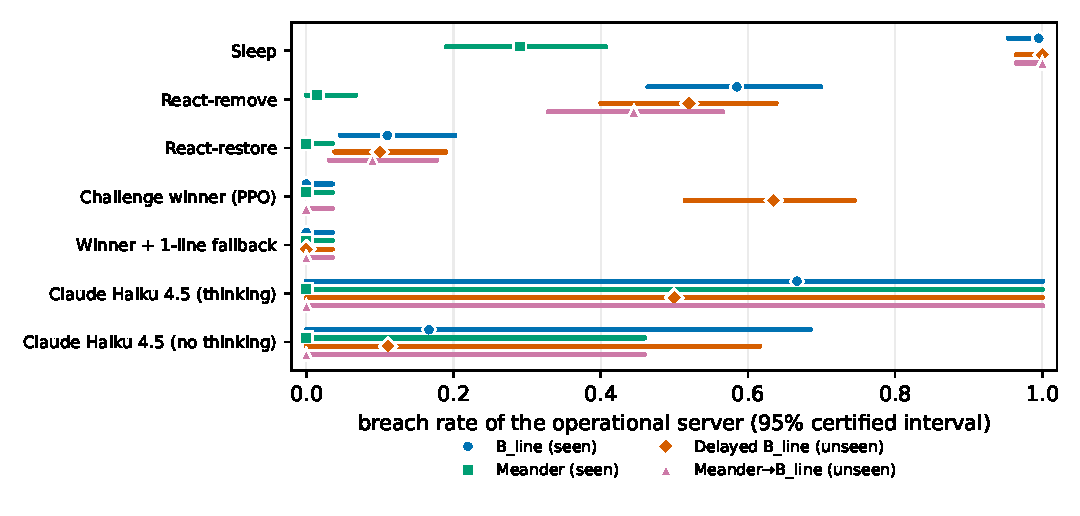
\includegraphics[width=\linewidth]{figure_breach_intervals.pdf}
\caption{Breach rate of the operational server per defender and attacker, with the
time-uniform 95\% certified interval. Non-LLM defenders: \CgEpisodes{} episodes per
attacker; LLM defenders: fewer (Table~\ref{tab:breach}), hence wider
intervals.}\label{fig:breach}
\end{figure}

\begin{figure}[t]\centering
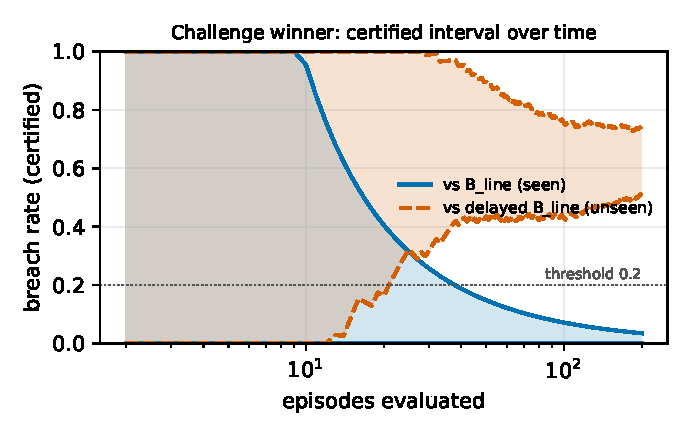
\includegraphics[width=0.95\linewidth]{figure_anytime.pdf}
\caption{The challenge winner's certified breach-rate interval as episodes accumulate,
against a seen attacker and against delayed B\_line. Bounds hold at every episode
count, so the evaluation may stop as soon as an interval clears the threshold.}\label{fig:anytime}
\end{figure}

\begin{table*}[t]\centering\footnotesize
\caption{Breach rate of the operational server: mean, and in parentheses the
time-uniform 95\% certified upper bound, per defender and attacker; $n$ episodes per
attacker. The adaptive attacker's bound is for the running average of its conditional
breach probabilities.}\label{tab:breach}
\begin{tabular}{@{}lrrrrrr@{}}\toprule
Defender & B\_line & Meander & Delayed B\_line & Meander$\to$B\_line & Adaptive & $n$\\\midrule
\tableinput table_cage_breach_rows.tex
\bottomrule\end{tabular}
\end{table*}

\begin{table}[t]\centering\footnotesize
\caption{Mean reward on the seen attackers and its rank, versus the certified worst-case
breach bound over the seen and over all fixed attackers and its rank (non-LLM defenders,
equal sample sizes), with the attacker attaining the worst case.}\label{tab:rank}
\begin{tabular}{@{}lrrrrrl@{}}\toprule
Defender & Mean & Rk & Seen & All & Rk & Worst\\\midrule
\tableinput table_cage_rank_rows.tex
\bottomrule\end{tabular}
\end{table}

\begin{table*}[t]\centering\footnotesize
\caption{LLM adaptive attacker: breach rate of the operational server (with the
time-uniform 95\% interval) against each defender, versus the best fixed strategy in
hindsight, uniform-random choice and the scripted EXP3 adversary, and the share of
episodes the model chose the best strategy.}\label{tab:attacker}
\begin{tabular}{@{}llrlrrrr@{}}\toprule
Model & Defender & $n$ & Breach (95\%) & Best & Rand. & EXP3 & Best-chosen\\\midrule
\tableinput table_cage_attacker_rows.tex
\bottomrule\end{tabular}
\end{table*}

\begin{figure}[t]\centering
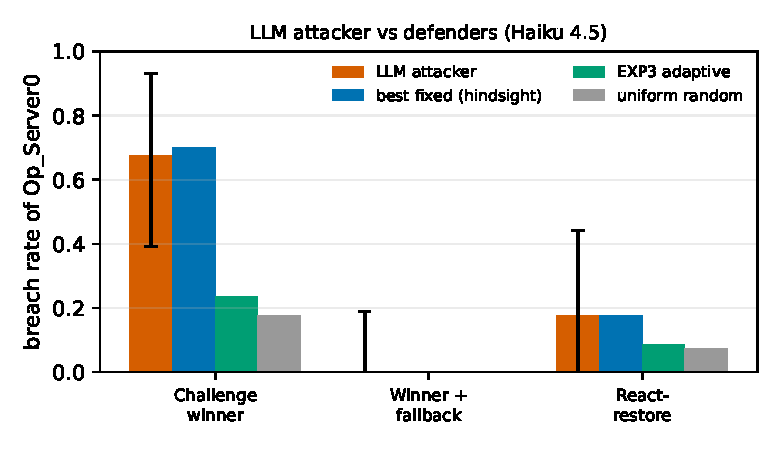
\includegraphics[width=0.92\linewidth]{figure_attacker.pdf}
\caption{LLM attacker (Haiku~4.5) breach rate per defender, with its 95\% certified
interval, next to the best fixed strategy in hindsight, the scripted EXP3 adversary and
uniform-random choice. The model matches the best fixed strategy against the winner and
is defeated by the one-line repair.}\label{fig:attacker}
\end{figure}

\begin{figure}[t]\centering
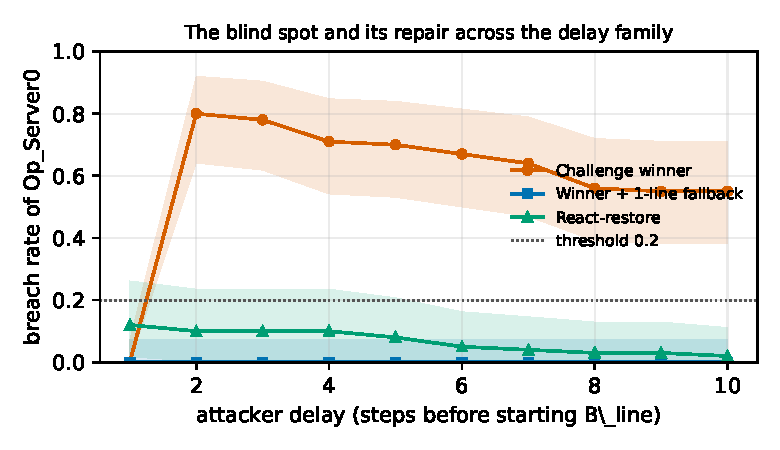
\includegraphics[width=0.92\linewidth]{figure_family.pdf}
\caption{Breach rate of the operational server against a B\_line that waits a fixed number
of steps before starting, with 95\% certified bands. The winner is safe at a one-step delay
but breached from two steps on, across the whole family; the one-line repair and
React-restore stay near zero.}\label{fig:family}
\end{figure}

\FloatBarrier
\section{Discussion}
Leaderboards that score agents against the attackers they were tuned on can certify
little about deployment: delaying an official attacker by one to five steps, using only
its own actions, defeats the strongest CAGE-2 agent. Certified worst-case evaluation over a
deliberately broadened attacker set catches this, names the failing attacker, and
measures whether a fix works. The same lens applies to the offence: a language model
told only to breach the defender rediscovers the winner's blind spot on its own and
exploits it harder than the scripted adaptive adversary, while the certified repair stops
it -- offence and defence judged on one scale. For LLM defenders the protocol makes a second point
concrete: their per-episode cost makes the number of episodes the binding constraint,
and time-uniform bounds let an evaluator spend only what a verdict requires.

\section{Limitations}
\paragraph{Simulation} CybORG Scenario~2 is a stylised network; results concern that
environment. Our second environment, CAGE Challenge~1, shares CybORG's engine and so is a
related rather than independent test of generality; a genuinely different simulator is
future work. \paragraph{Worst case over a set} Certificates hold over the attackers we
include, not all attackers; our unseen attackers are deliberately simple. \paragraph{Port}
The winner is evaluated through our NumPy port; it reproduces the published Meander
score but not the B\_line score, which we attribute to the authors' unpublished
environment change. The delayed-start failure does not rest on that score: it is driven
by the winner's own released attacker-selection rule -- the delay makes its early-scan
fingerprint match neither trained policy, so it loads the sleep policy and does nothing --
a property of the published decision logic, not of our port's absolute B\_line reward. \paragraph{LLM evaluation} Few episodes per attacker, one prompt, and the
command-line interface's default sampling; the LLM results are descriptive and their
certified bounds are wide. Every language model we evaluate, as defender and as
attacker, is a Claude model from a single vendor -- the family that also assisted with
this work's code -- so nothing here speaks to how models from other families behave.
\paragraph{Budget control} Parallel workers check a shared spending cap before each
episode, so a run can exceed its cap by up to one episode per worker; the Sonnet run
did. \paragraph{Attacker scope} The two attackers test different things: the strategy selector
supplies adaptation over ready-made attacks, and the primitive attacker operates the kill
chain through CybORG's action abstraction -- still not raw network exploitation (no packet
crafting or novel vulnerability discovery), which the simulator does not model. \paragraph{Price of anytime validity} Time-uniform bounds are wider than fixed-sample
tests at small $n$; we report conventional paired tests alongside where relevant.

\paragraph{Artifact and AI use} Third-party code (CybORG, the winning agent) is fetched at
pinned commits with hash-checked weights. All numbers are generated from committed
tables; LLM transcripts and costs are recorded per episode. The analysis code and draft
text were produced with the assistance of an AI system (Claude); results are reproduced
by automated tests.

\begin{thebibliography}{99}
\bibitem{standen2021cyborg} M.~Standen, M.~Lucas, D.~Bowman, T.~J. Richer, J.~Kim, and
D.~Marriott. CybORG: A gym for the development of autonomous cyber agents.
arXiv:2108.09118, 2021.
\bibitem{castro2025llm} S.~R. Castro, R.~Campbell, N.~Lau, O.~Villalobos, J.~Duan, and
A.~A. Cardenas. Large language models are autonomous cyber defenders. In \emph{IEEE
Conference on Artificial Intelligence (CAI)}, 2025. arXiv:2505.04843.
\bibitem{king2025graph} I.~J. King, B.~Bowman, and H.~H. Huang. Automated cyber defense
with generalizable graph-based reinforcement learning agents. arXiv:2509.16151, 2025.
\bibitem{hannay2022cardiff} J.~Hannay. CAGE Challenge 2 winning agent: PPO with greedy
decoys. Source code and report, 2022.
\bibitem{hammar2024optimal} K.~Hammar, N.~Dhir, and R.~Stadler. Optimal defender
strategies for CAGE-2 using causal modeling and tree search. arXiv:2407.11070, 2024.
\bibitem{palmer2025egta} G.~Palmer, L.~Swaby, D.~J.~B. Harrold, M.~Stewart, A.~Hiles,
C.~Willis, I.~Miles, and S.~Farmer. An empirical game-theoretic analysis of autonomous
cyber-defence agents. arXiv:2501.19206, 2025.
\bibitem{waudbysmith2023betting} I.~Waudby-Smith and A.~Ramdas. Estimating means of
bounded random variables by betting. \emph{Journal of the Royal Statistical Society
Series B}, 2023.
\bibitem{howard2021timeuniform} S.~R. Howard, A.~Ramdas, J.~McAuliffe, and J.~Sekhon.
Time-uniform, nonparametric, nonasymptotic confidence sequences. \emph{Annals of
Statistics}, 2021.
\bibitem{auer2002exp3} P.~Auer, N.~Cesa-Bianchi, Y.~Freund, and R.~E. Schapire. The
nonstochastic multiarmed bandit problem. \emph{SIAM Journal on Computing}, 2002.
\end{thebibliography}

\end{document}
